% Muster f�r die Seminarausarbeitung
% HPI Potsdam

\documentclass[11pt, a4paper]{article}


\usepackage[english]{babel}
\usepackage[latin1]{inputenc} %Korrekte Kodierung der Umlaute nach ISO 8859-1
\usepackage[T1]{fontenc} %Korrekte Kodierung der Umlaute nach ISO 8859-1
\usepackage{makeidx} %Zur automatischen Indexerstellung
\usepackage{amsfonts}
\usepackage{amsmath}
\usepackage{amssymb}
\usepackage{epsfig}   % Zum Einbinden von Bildern
\usepackage{url}      % Korrekter Satz von URLs
\usepackage{color}    % Verwendung von Farben
\usepackage{listings} % Korrekter Satz von Listings und Quellcode
\usepackage{wrapfig}
\usepackage{todonotes}
\usepackage[numbers,round]{natbib}

%Hilfs-Fonts - ohne Serifen (hier f�r Tabellen)
\newfont{\bib}{cmss8 scaled 1040}
\newfont{\bibf}{cmssbx8 scaled 1040}

\definecolor{lightgray}{gray}{0.85}

%Seitenformat-Definitionen
\topmargin0mm
\textwidth147mm
\textheight214mm
\evensidemargin5mm
\oddsidemargin5mm
\footskip19mm
\parindent=0in

\makeindex % legt das Index-File an


\begin{document}

\begin{titlepage}
  \begin{center}
    \mbox{}
    \vspace{1cm}

    {\huge Semantic and Visual Image Clustering\\[1em] {\LARGE Retrieving Search Term Related Pictures in Structured Clusters}}

    \vspace{4.7cm}

    Seminar paper \\[1em]
    {\large \sc Semantic Multimedia} \\[1em]
    Summer Term 2013 \\[1em]
    Hasso-Plattner-Institut f�r Softwaresystemtechnik GmbH \\[1em]
    Universit�t Potsdam

    \vspace{3.7cm}

		written by
		
    \vspace{1em}

		{\Large Mandy Roick} \\
		{\Large Claudia Exeler} \\
		{\Large Tino Junge} \\
		{\Large Nicolas Fricke}
		
    \vspace{4em}

    30.~August 2013
  \end{center}
\end{titlepage}


\setcounter{page}{1}

% Zweite Seite = Kurzzusammenfassung
\begin{center}
{\bf Abstract}
\end{center}

\noindent
\todo{Write the abstract}
Abstract goes here.

\bigskip

Write it at the end.

\newpage

% Dritte Seite = Inhaltsverzeichnis
\tableofcontents
\newpage

\listoftodos
\newpage

\section{Retrieving Images in Clusters}
\label{sec_introduction}

\todo{introduce the introduction?}

\subsection{Problem Statement \& Motivation}
training data for image categorization and content detection \\
flickr and other online photo communities are good sources for annotated images \\
problems: low annotation quality, only search for specific term (with different meanings and visual characteristics) \\
for example, want to test the quality of my algorithm in identifying different foods: would have to think of all kinds of food and search and filter images manually

\bigskip

\emph{What do we do?} \\
clustering: creating homogeneous groups of semantically and visually similar pictures \\

\emph{Why do we do that?} \\
seminar challenge: cluster 1 million pictures of the MIR1M flickr file set \\
improving the complex task of searching for pictures according to a given keyword \\
facing different challenges like: multiple meanings of the keyword, bad picture annotations, taking semantic and visual information of a picture into account \\

\subsection{Clustered Tree Nodes Approach}
idea: provide ready-to-use semantically and visually homogeneous image clusters for a given topic. Span tree of subordinate pictures, retrieve related images and cluster them to distinguish different settings of the pictures and to identify outliers.

Implemented a web application in Python

\bigskip

After giving an overview of Related Work in chapter 2, we will present our methods for retrieving (chapter 3) and clustering (chapter 4) appropriate images. Chapter 5 explains how we evaluate our approach, while the evaluation results will be discussed in chapter 6. At last, chapter 7 gives ideas for improvement and possible future work.

\newpage
\section{Related Work}
\label{sec_relatedwork}

Much research has been done recently in image clustering and semantic clustering, with application areas in image segmentation, compact representation of large image sets, search space reduction and avoiding the semantic gap in content based image retrieval \cite{Lim2011}.
However, most of these works present new algorithms for one of the above use cases, not methods to retrieve training data. 

\bigskip
The only algorithm for retrieving training data for image analysis was found in \cite{Orendovici2010}. The algorithm collects training data for computational analysis of the quality of photographs from Flickr. But, instead of analyzing pictures automatically according to their tags and comments, the paper presents a tool for collecting user votes. Comments were only used to retrieve terms for describing image quality.

\bigskip
Related Subjects: Image Annotation, semantic clustering, content-based image retrieval

\subsection{Semantic Clustering and Tags}
The idea of clustering search results based on tags and other annotations has been implemented before by \cite{Ramage2009} but for web pages instead of images. The main difference is that documents such as web pages consist of words, so their content itself can be used for semantic analysis.
Current issues with tag-based search and clustering are mostly related to the lack of a defined tag vocabulary (e.g. the use of synonyms, homonyms, variations in spelling etc.), and elaborated on more closely in \cite{Auer2011}.

\subsection{Image Annotation and Content-Based Image Retrieval}
%% ?? http://ganges.usc.edu/pgroupW/images/6/6b/Cvm2012.pdf: detect objects and organize images based on the relations of the objects within.
%% http://ieeexplore.ieee.org/xpls/abs_all.jsp?arnumber=718510: review of visual features for cbir

Ideas exist to use visual features to semantically analyze and classify images. \cite{Liu2007} and \cite{Zhang2012} provide good summaries and evaluations of the different approaches how this could be done. Both conclude that this so-called \emph{Automatic Image Annotation} \index{Automatic Image Annotation} is computation-intensive and not yet fully mature.

%% http://infolab.stanford.edu/~wangz/project/imsearch/review/MTA/neela.pdf: summary of semantic image interpretation; Overview of foundations
\bigskip
One approach that combines semantics and visuals to analyse pictures in a so called \emph{visual folksonomy} is \cite{Lindstaedt2009}, which tries to annotate images, with a controlled vocabulary, based on visual features and existing tags. Their goal, however, is to create additional annotations for not or poorly tagged images. Another approach is presented by \cite{cai2004hierarchical} with the aim to cluster images returned by a WWW image search. In contrast to pictures from a folksonomy, image search results are connected to a web page with context and link information which is used by the algorithm to cluster images.

\newpage
%
\section{Image Tree Based on Wordnet}
\label{sec_wordnetsearchtree}

\subsection{Wordnet}\index{Wordnet}
The offical web page (ref: http://wordnet.princeton.edu/) describes WordNet as a freely and publicly available "large lexical database of english nouns, verbs, adjectives and adverbs, grouped into sets of cognitive synonyms (synsets), each expressing a distinct concept." That is, a synset is a particular concept, that can be expressed by different terms but has one unique identifier. The identifier consists of of the word most commonly used to describe the concept, the part of speech, and a number, e.g. \emph{drive.v.02}.
The number is necessary because one word can have multiple meanings that will then be represented by different synsets, like in \emph{cherry.n.01} for the tree and \emph{cherry.n.02} for the fruit. \\

Synsets are linked with each other through several semantic relations, e.g. hyponyms or meronyms. \\
In our work, we use this network of synsets to discover the semantics between terms describing the images as well as towards the search term. \\
  

\subsection{Constructing a Searchtree}
two typical types of queries: more or less generic object descriptors, and places \\
actually construct multiple searchtrees if more than one synset found for a searchterm (i.e. train coach and motorized vehicle for car)\\
use hyponym relation to span tree of specializations (i.e. apple, banana for fruit; bus, sportscar for car)\\
if no hyponyms (usually the case for geographic terms), use part-meronyms\\

\subsection{Synset Detection}
for each tag and word in title, try to find synset (limiting ourselves to nouns, because they are usually the ones describing the depicted concepts). Further source options: description (named entity recognition necessary), comments (noticed little relation to picture), group and album names (for both preprocessing needed to match any to wordnet)  \\
problem: multiple possible synsets for a word, how to find correct meaning? \\
use best-first search (with limited queue for complexity reasons. idea is that paths at more than position x are unlikely to become best candidate anyways) \\
still erroneous with words that are meant in a way that is unknown to WordNet, i.e. canon as the camera model is interpreted as [definition of canon.n.01]  \\
therefore preprocessing removes all tags that include numbers. Blacklist could filter even more but would also filter canon in its real sense, and generally not desirable to be flexible with respect to the tag vocabulary.  \\
also removes special characters (more likely to be found on WordNet, and more likely to be identical with other unmatchable tags) 
problem: multiple possible synsets for a word, how to find correct meaning? \\
use best-first search with limited queue, distances are based on Leacock and Chodorows Normalized Path Length (lch similarities, which is perceived as closer to human understanding than regular path similarity \cite{budanitsky01} )

\subsection{Assigning Pictures to Tree Nodes}
for higher recall: find strongly co-occurring tags that could not be mapped to synset \\
strong co-occurrence defined on tf-idf (else camera models would be strong co-occurrence with many synsets)
observed that it is useful to find translations etc. but of course also introduces noise \\
take all pictures that are annotated with at least one of the related tags or the synset itself.

\newpage
%
\section{Semantic and Visual Clustering}
\label{sec_inhalt}

The nodes received through the tree-based search are potentially very large (i.e., many pictures were found for the node). We found a rather small semantic and a large visual diversity within these nodes. It is therefore appropriate to refine especially the large nodes into smaller clusters.

\subsection{General Approach}
Since semantics are more meaningful to humans, and thus likely to be more important for the given use case, the refinement is done first on a semantic and then on a visual basis. That is, the results from the groups with semantically similar pictures are clustered again into subclusters with visually similar pictures. The steps are explained in more detail in sections \ref{sec_keywordclustering} and \ref{sec_visualclustering}.
This approach has the additional advantage that outlier images, which have been assigned to a node but do not quite fit with the others because they show something different, can be filtered out in the semantic step. \\
The subclustering explained below and summarized in figure \ref{fig_semanticandvisual} will only take place for nodes/clusters with a certain minimum size and results in the structure of three nested Arrays of the WordnetNode class' attribute \emph{subclusters} shown in figure \ref{fig_nodestructure}.

\todo{add Search Term to graphic}
\begin{figure}[h]
\centering
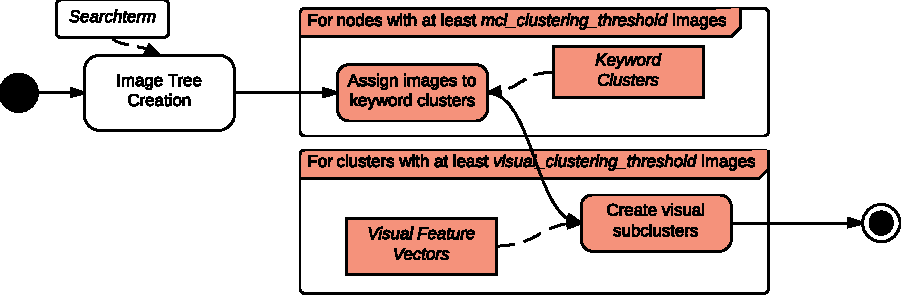
\includegraphics[width=\textwidth]{images/semantic_and_visual_clustering.pdf}
\caption{Process of Semantic and Visual Clustering}
\label{fig_semanticandvisual}
\end{figure}

The data structures used in the process, such as Image Lookup Structures and Visual Feature Vectors, need only be calculated once for each image set. The preparational processes are visualized by figure \ref{fig_precalcprocess}.

\begin{figure}[h]
\centering
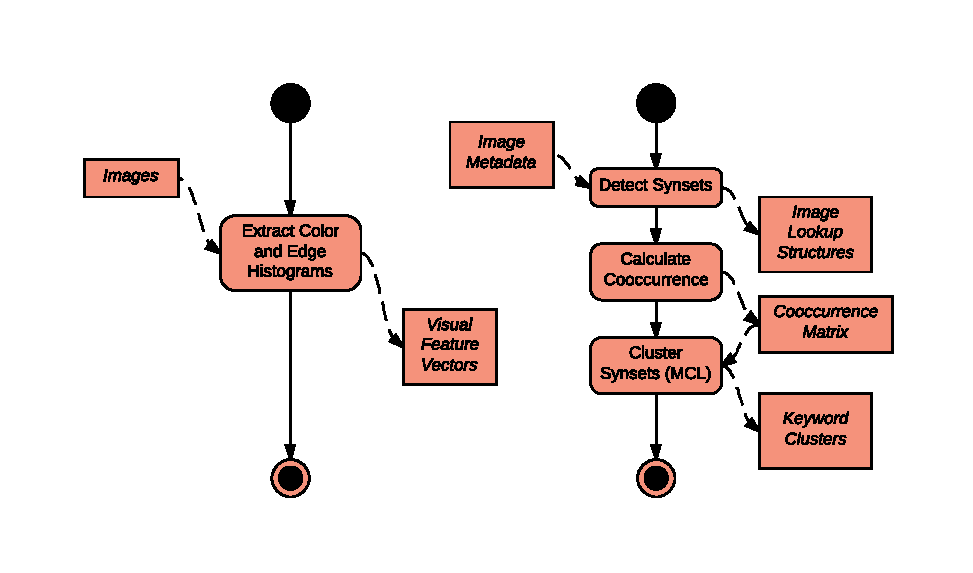
\includegraphics[width=0.8\textwidth]{images/precalcs_activity_diagram.pdf}
\caption{Static structures creation processes}
\label{fig_precalcprocess}
\end{figure}


\subsection{Keyword Clusters}
\label{sec_keywordclustering}
Semantic clustering is accomplished by using the associated Synsets which the Synset detection assigned to each image (see chapter \ref{sec_synsetdetection}). Therefor, Synsets are clustered into groups and images are assigned to these groups.

\bigskip
The paper ``Automated Tag Clustering'' by Grigory Begelman \cite{begelman2006automated} presents an algorithm for tag clustering based on graph clustering. It uses co-occurrences of tags to span a graph whose nodes represent tags and whose edges represent co-occurrences. We adapt the algorithm to include the advantages of WordNet. That is why, we replace the number of co-occurrences by a combination of co-occurrences and LCH-Similarity\index{LCH-Similarity}.
A disadvantage of this algorithm is the graph clustering via eigenvalues and eigenvectors that is expensive for large graphs. Furthermore, this algorithm does not take edge weighting into account.

Consequently, we replace the graph clustering algorithm by the Markov Cluster Algorithm (MCL)\index{Markov Cluster Algorithm} introduced by Dongen \cite{Dongen1998}. MCL is based on the Random Walk Model \cite{spitzer2001principles}. The basic idea is, if you start to walk from a node, it is more likely to stay inside a cluster than to leave it. Therefore, we calculate the probability to reach a node $B$ from another node $A$ in only one step. Then, we walk steps through the graph until the probabilities converge. The resulting probabilities inside a cluster are higher than outside. So, they can be used to determine groups of related Synsets.

\bigskip
To assign images to Synset clusters, we count how many Synsets the image shares with each cluster. It is then assigned to the cluster with the most matching Synsets. If two clusters have the same number of matching Synsets, the image is assigned to both clusters. As a consequence, a semantic cluster consists of images which have many associated Synsets in the same Synset cluster. For example, some pictures with parrots fall into a Synset cluster with persons, others in those with trees.

\bigskip
The advantages of an additional semantic clustering in each node of the image tree are obvious when looking at ``Africa'' as search term. The spanned tree consists of part-meronyms which are the countries of Africa. However, the pictures show people, animals, vegetation, cities, or other content not related solely to Africa. Simply with the help of the image tree, it is not possible to separate between those categories. Semantic clustering, allows in this context a more fine grained clustering. Also, in a well separated tree it is possible to achieve a more fine grained clustering. Pictures of the tree node \emph{parrot.n.01} could be separated into pictures showing parrots in nature and pictures showing parrots in a zoo.

Furthermore, semantic clustering permits the detection of outliers. If too few images fall into the same semantic cluster, they are considered to be outliers, and they are deleted from the tree node. For instance, a picture showing a cat whose name is ``Alexandria'', which is a city in Africa, can be deleted from the tree for the search term ``Africa''.

\subsection{Visual Clusters}
\label{sec_visualclustering}

One difficulty in the visual part of our work, besides the choice of appropriate features and their implementation, is the question how to use them jointly in a suitable algorithm for clustering.

\subsubsection{Features}
The features we chose for our tool are:
\begin{itemize}
\item{Color histogram} in HSV color space with 20 bins (i.e., 20 ranges) each
\item{Edge histogram} length and angle histograms with 10 bins (i.e., 10 different angles considered) as combined vector
\end{itemize}
The reasons we chose these are that they are easy to calculate, rather obvious and humanly comprehensible. Since the purpose of this visual clustering is only in refining the semantic clusters, and not in trying to distinguish concepts by visual features, there is no apparent need for the use of more complex features.\\
For feature extraction, we use a pyramidal approach similar to the one proposed in \cite{Lazebnik2006}. Its advantage is that it combines features extracted over the entire image with features extracted on separate regions. The advantage of splitting images into regions for feature extraction is that, for example, two images with the same colors but in different structures will not automatically have the same color feature vectors (as visualized in figure \ref{fig_blackwhite}). At the same time, the images' structure gains an unproportionally high importance, especially when using a large number of regions. When using 5x5 rectangles, for example, it can be observed that images with same-colored borders were considered very similar, independent of their actual content.

\begin{figure}[h]
\centering
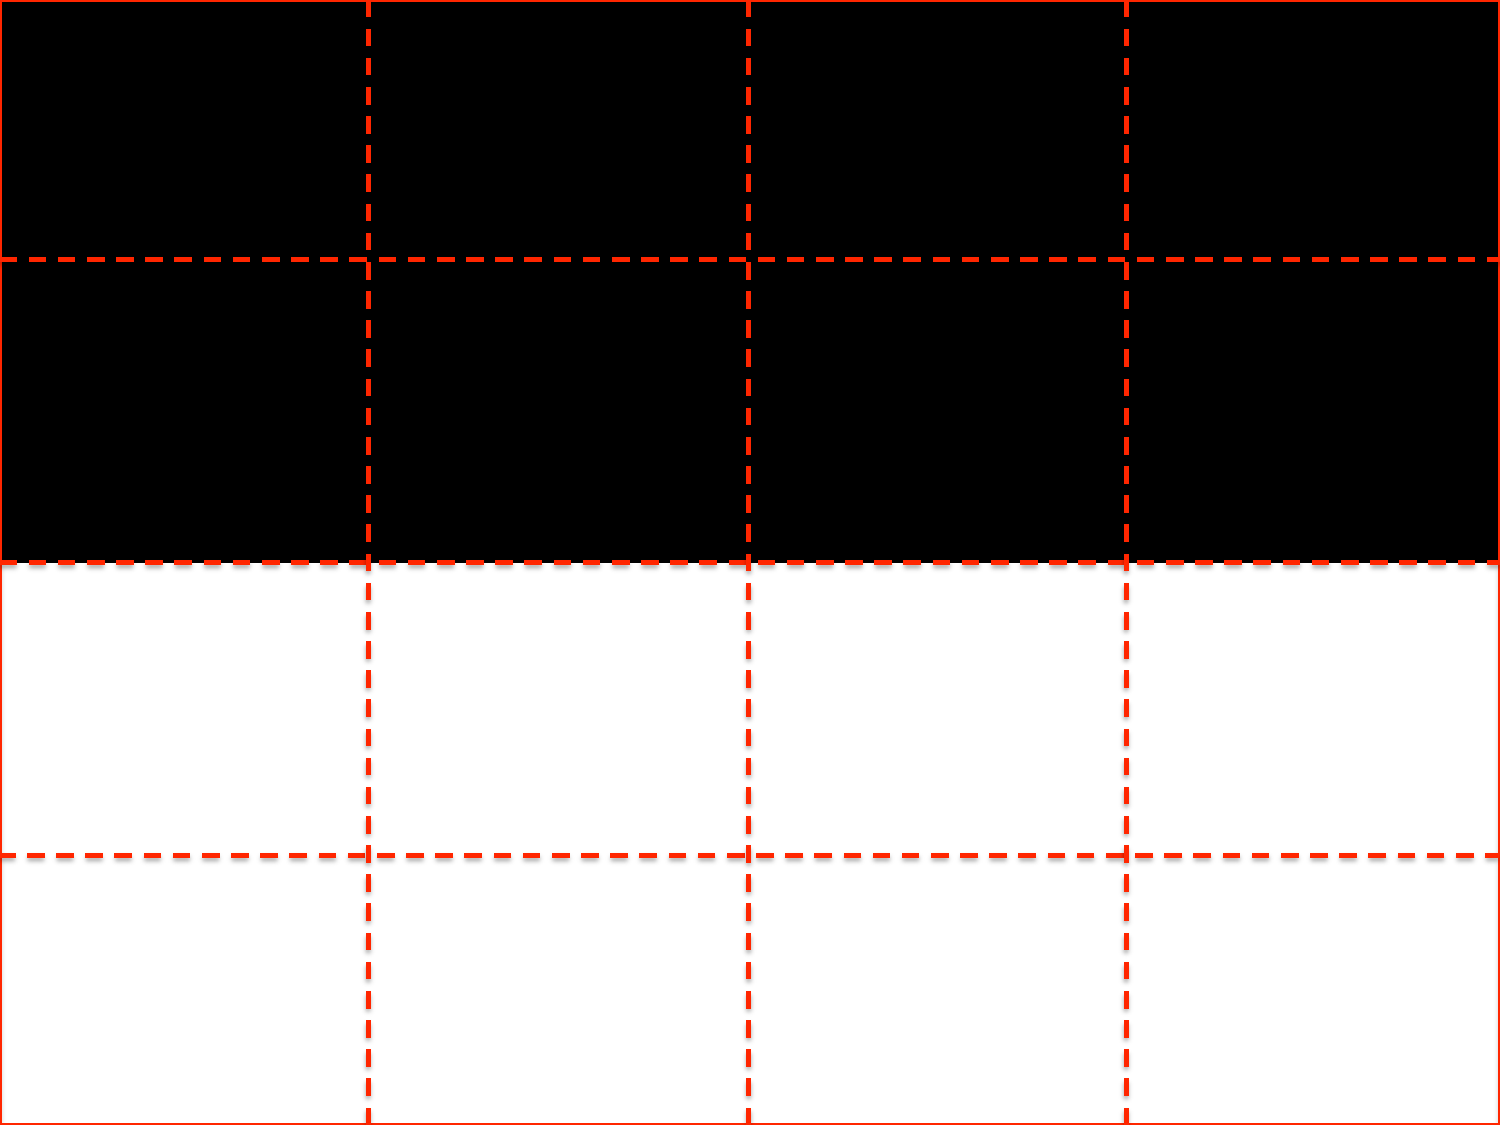
\includegraphics[width=0.35\textwidth]{images/blackwhite1.pdf}

\includegraphics[width=0.35\textwidth]{images/blackwhite2.pdf}
\caption{Two images that have the same color histogram regarding the entire picture but different histograms on the marked regions}
\label{fig_blackwhite}
\end{figure}

With the applied pyramid technique, the final feature vector is concatenated from several partial feature vectors, labeled from 1 to 30 in figure \ref{fig_blackwhite}. The appropriateness of this method especially for refining existing clusters, is also discussed in \cite{Lazebnik2006}.

\begin{figure}[h]
\centering
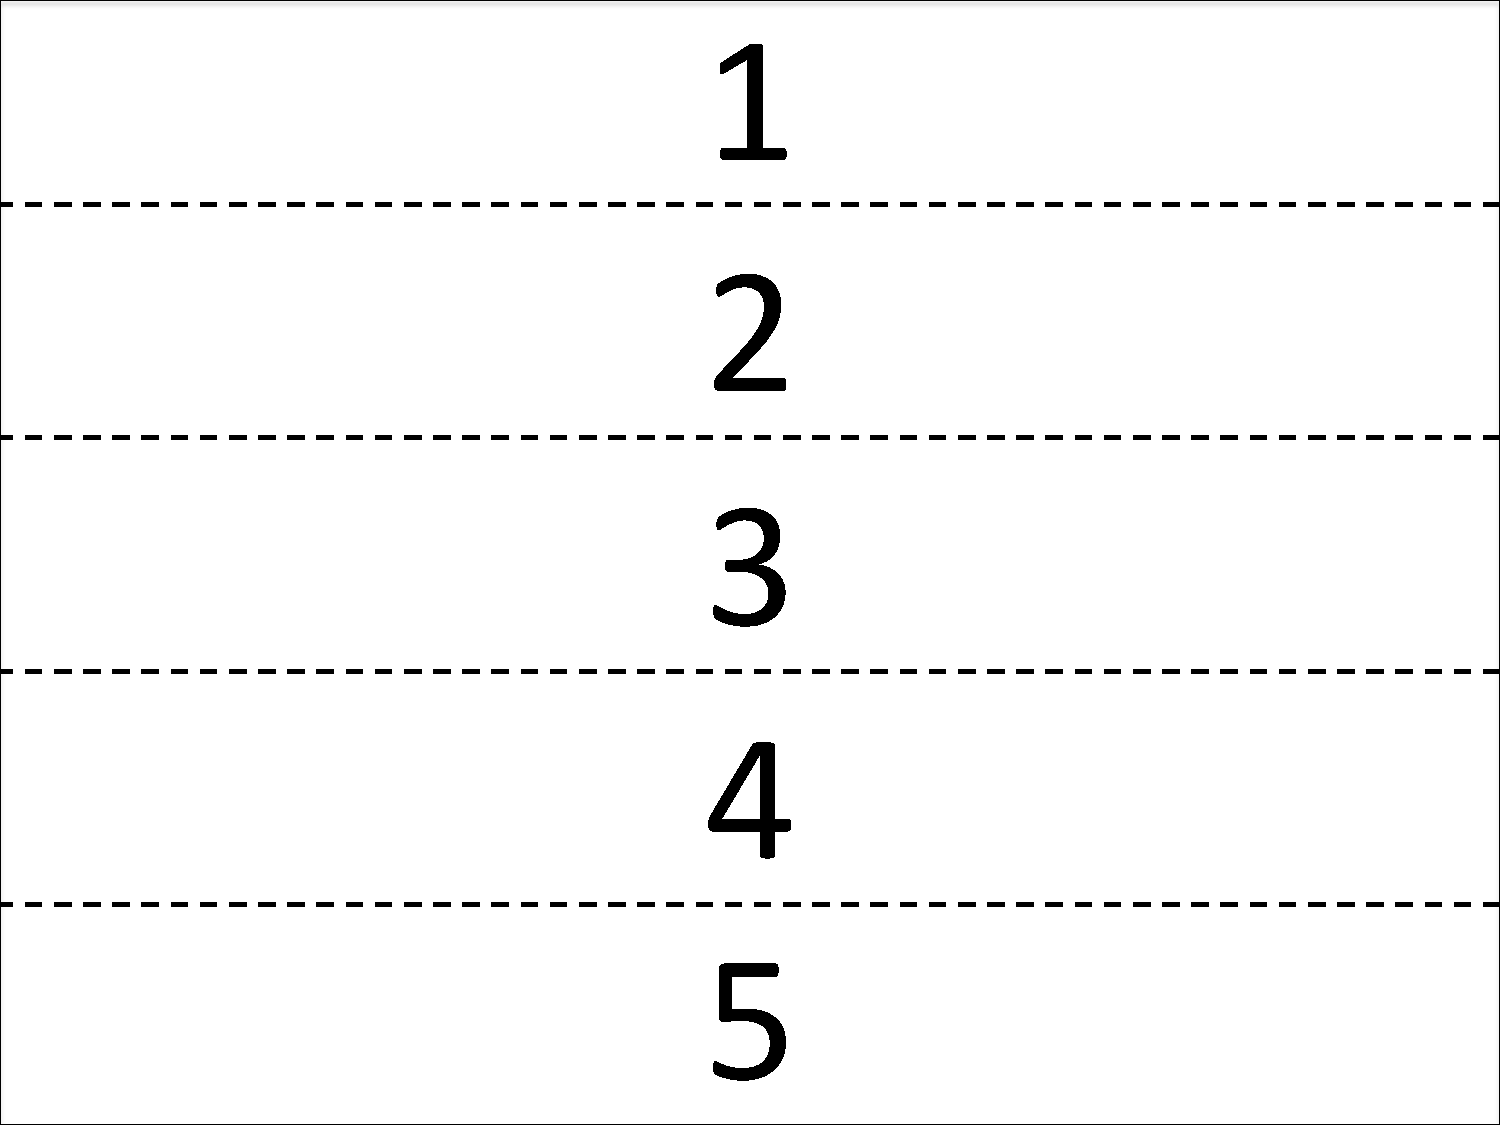
\includegraphics[width=0.19\textwidth]{images/partitioning5h.pdf}
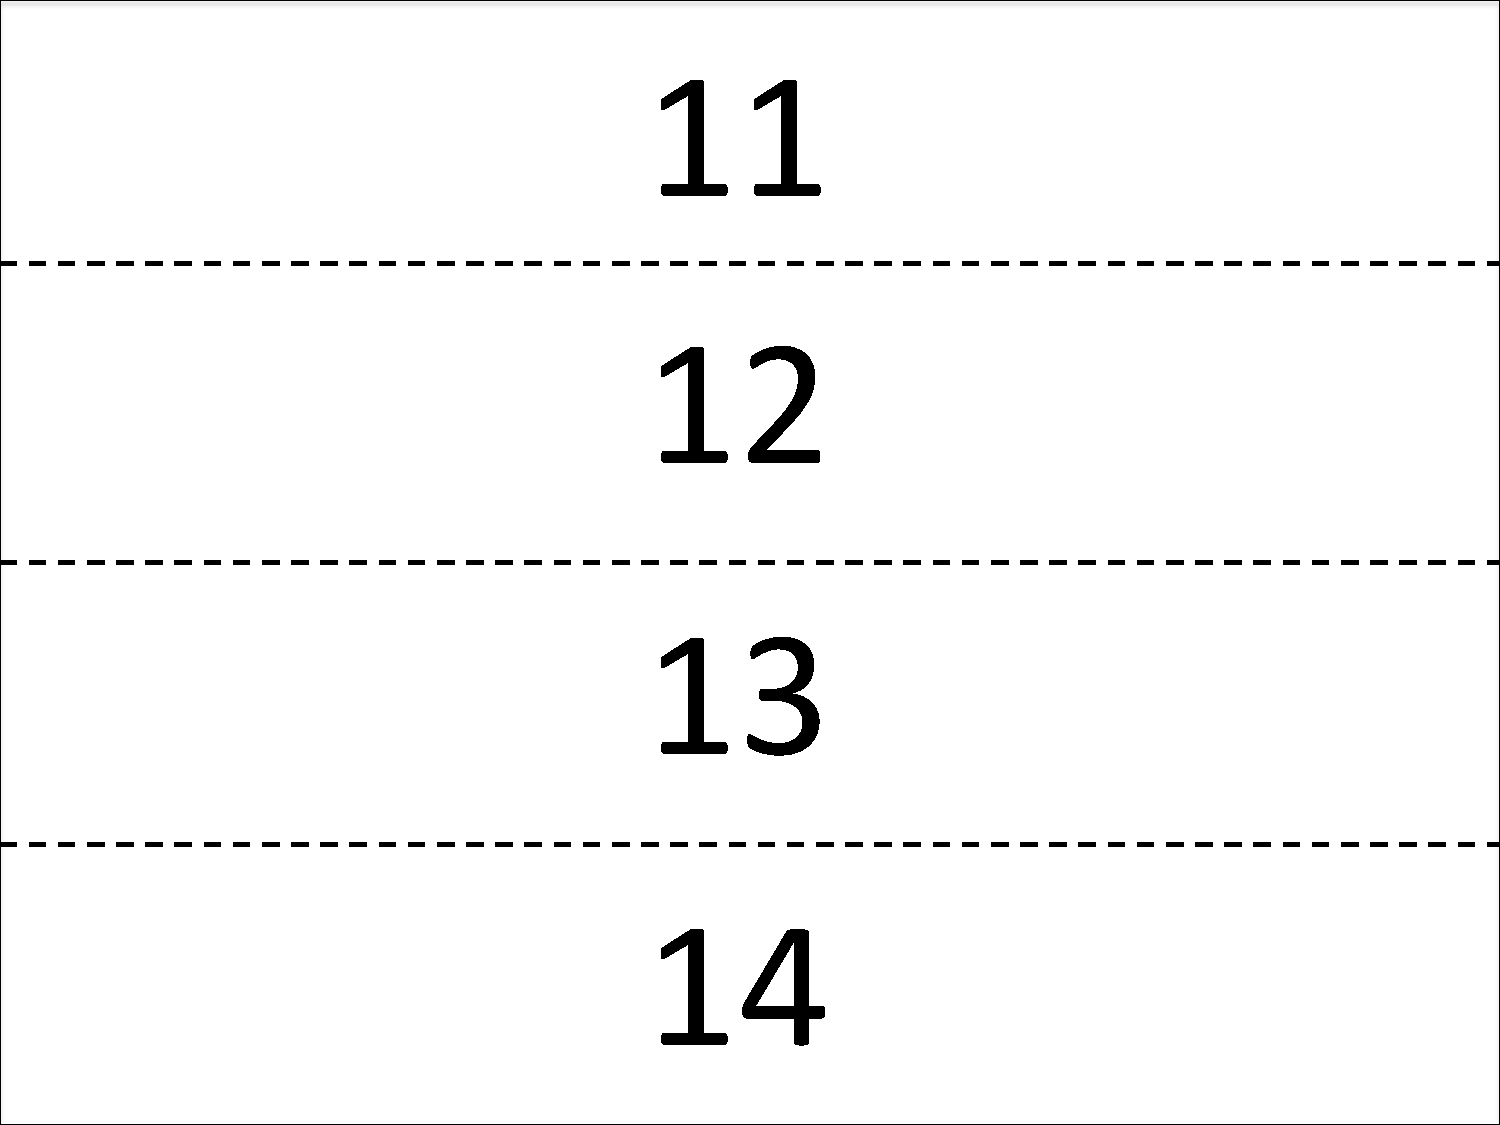
\includegraphics[width=0.19\textwidth]{images/partitioning4h.pdf}
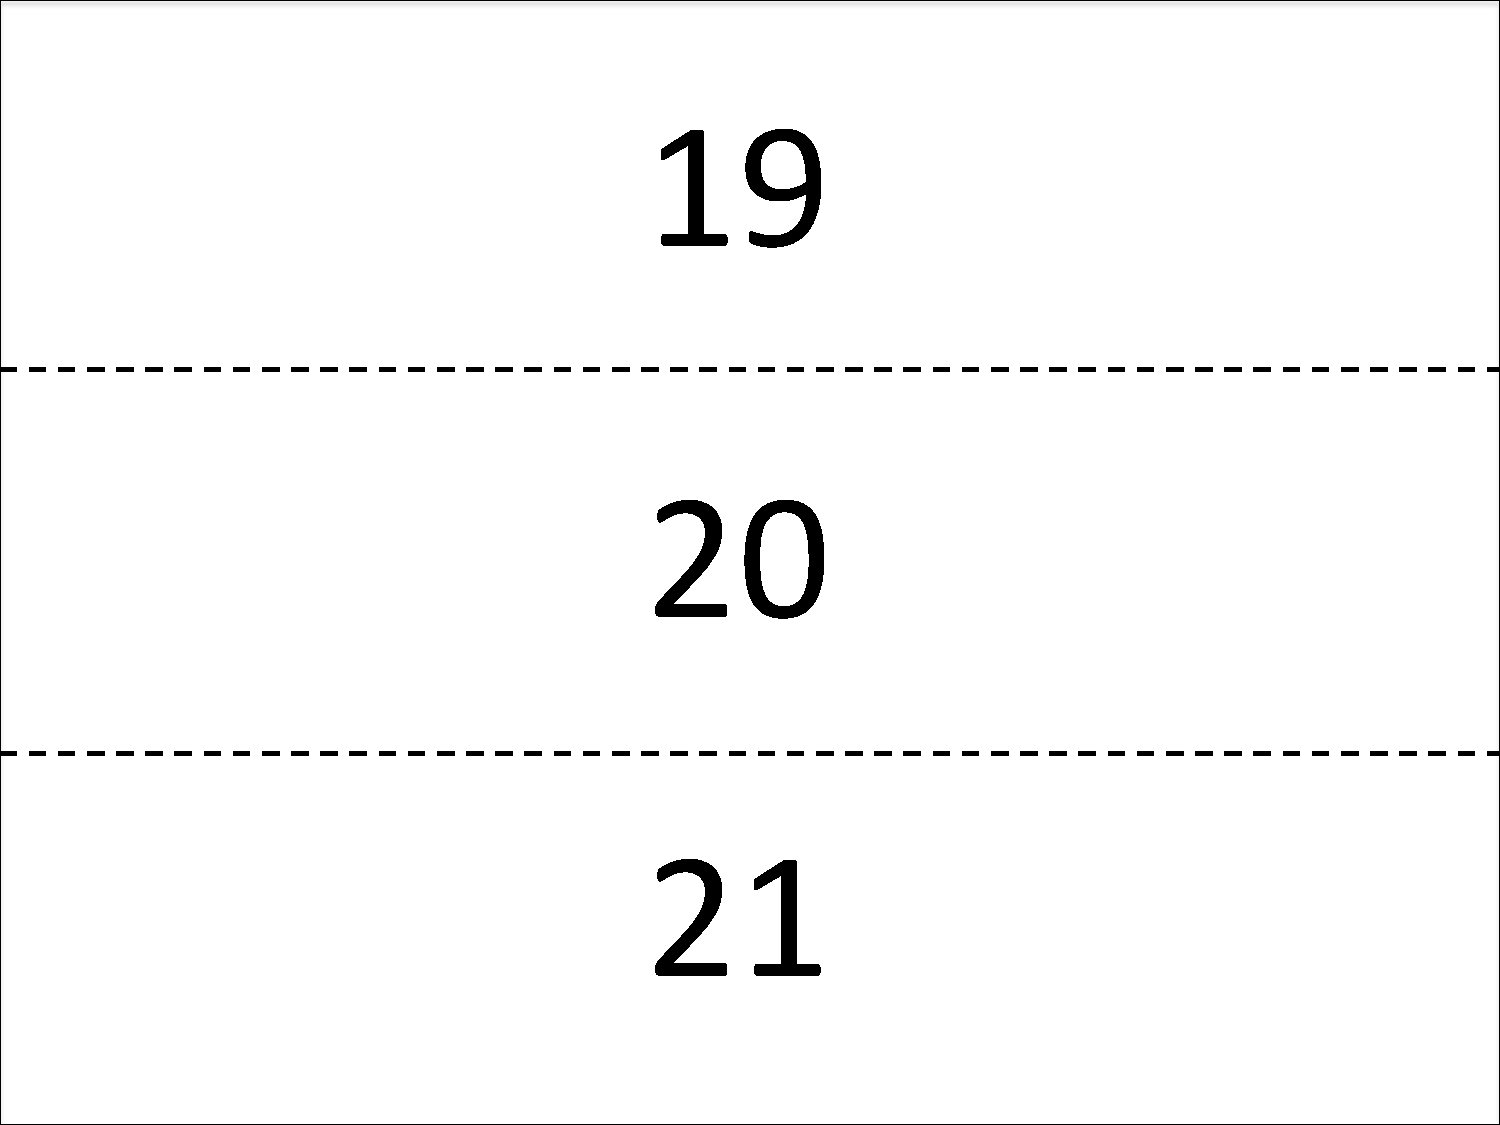
\includegraphics[width=0.19\textwidth]{images/partitioning3h.pdf}
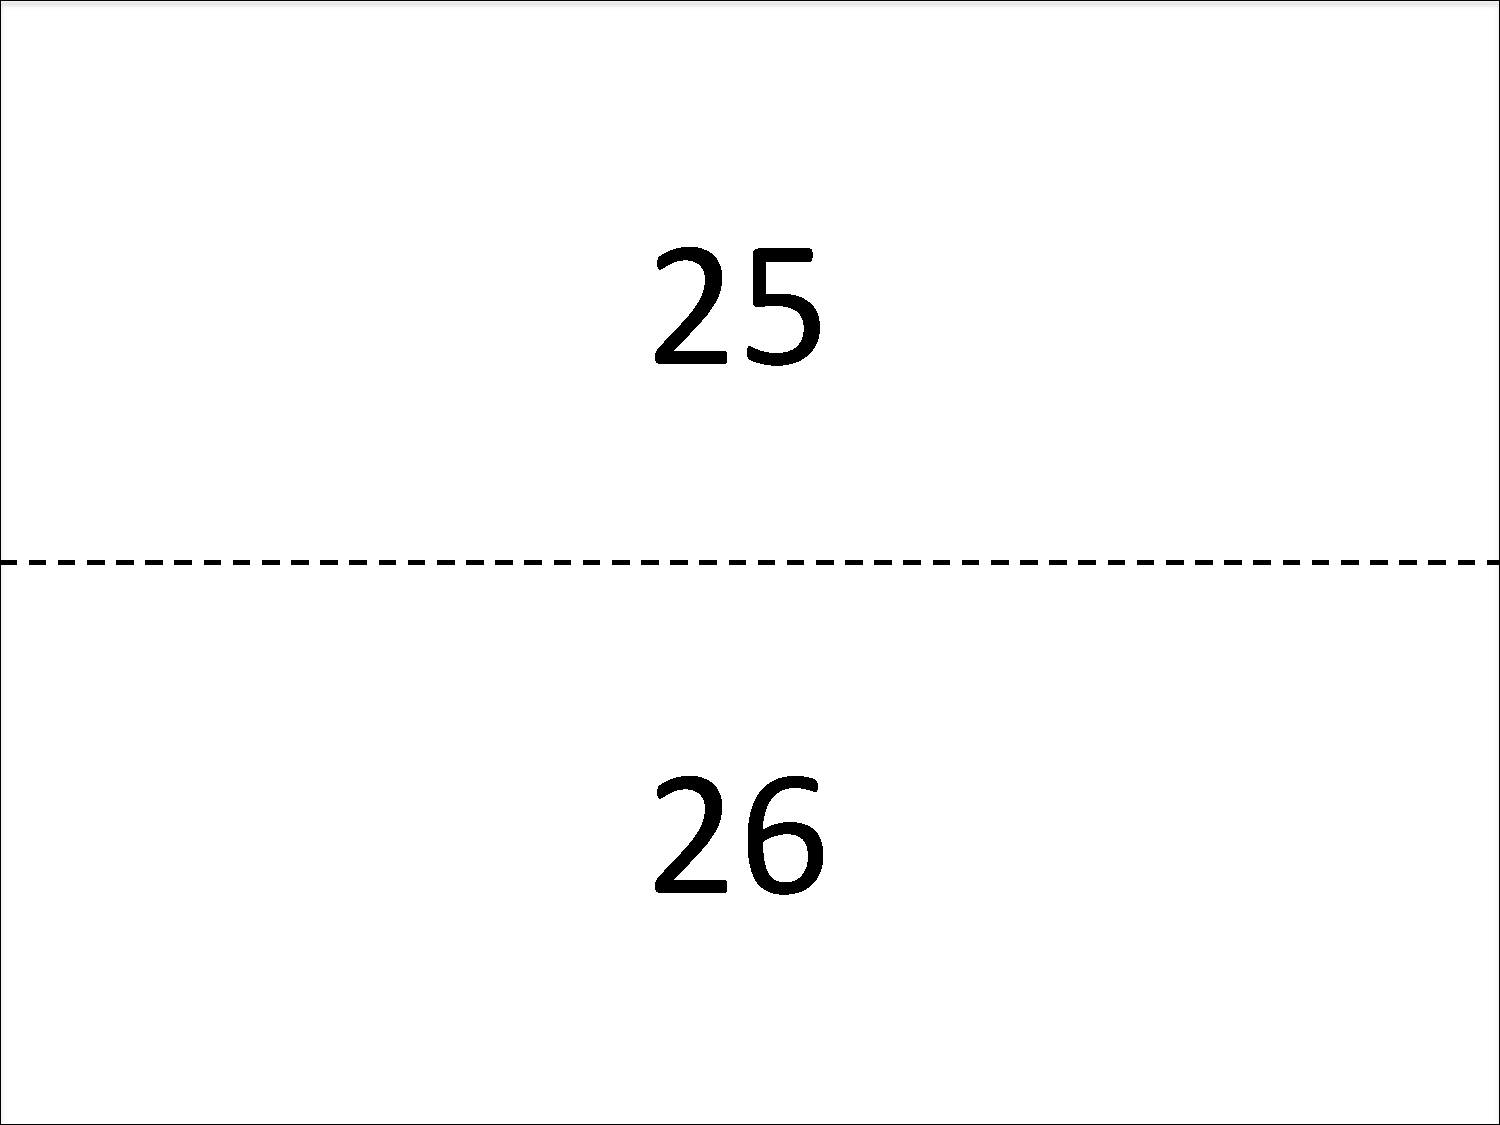
\includegraphics[width=0.19\textwidth]{images/partitioning2h.pdf}
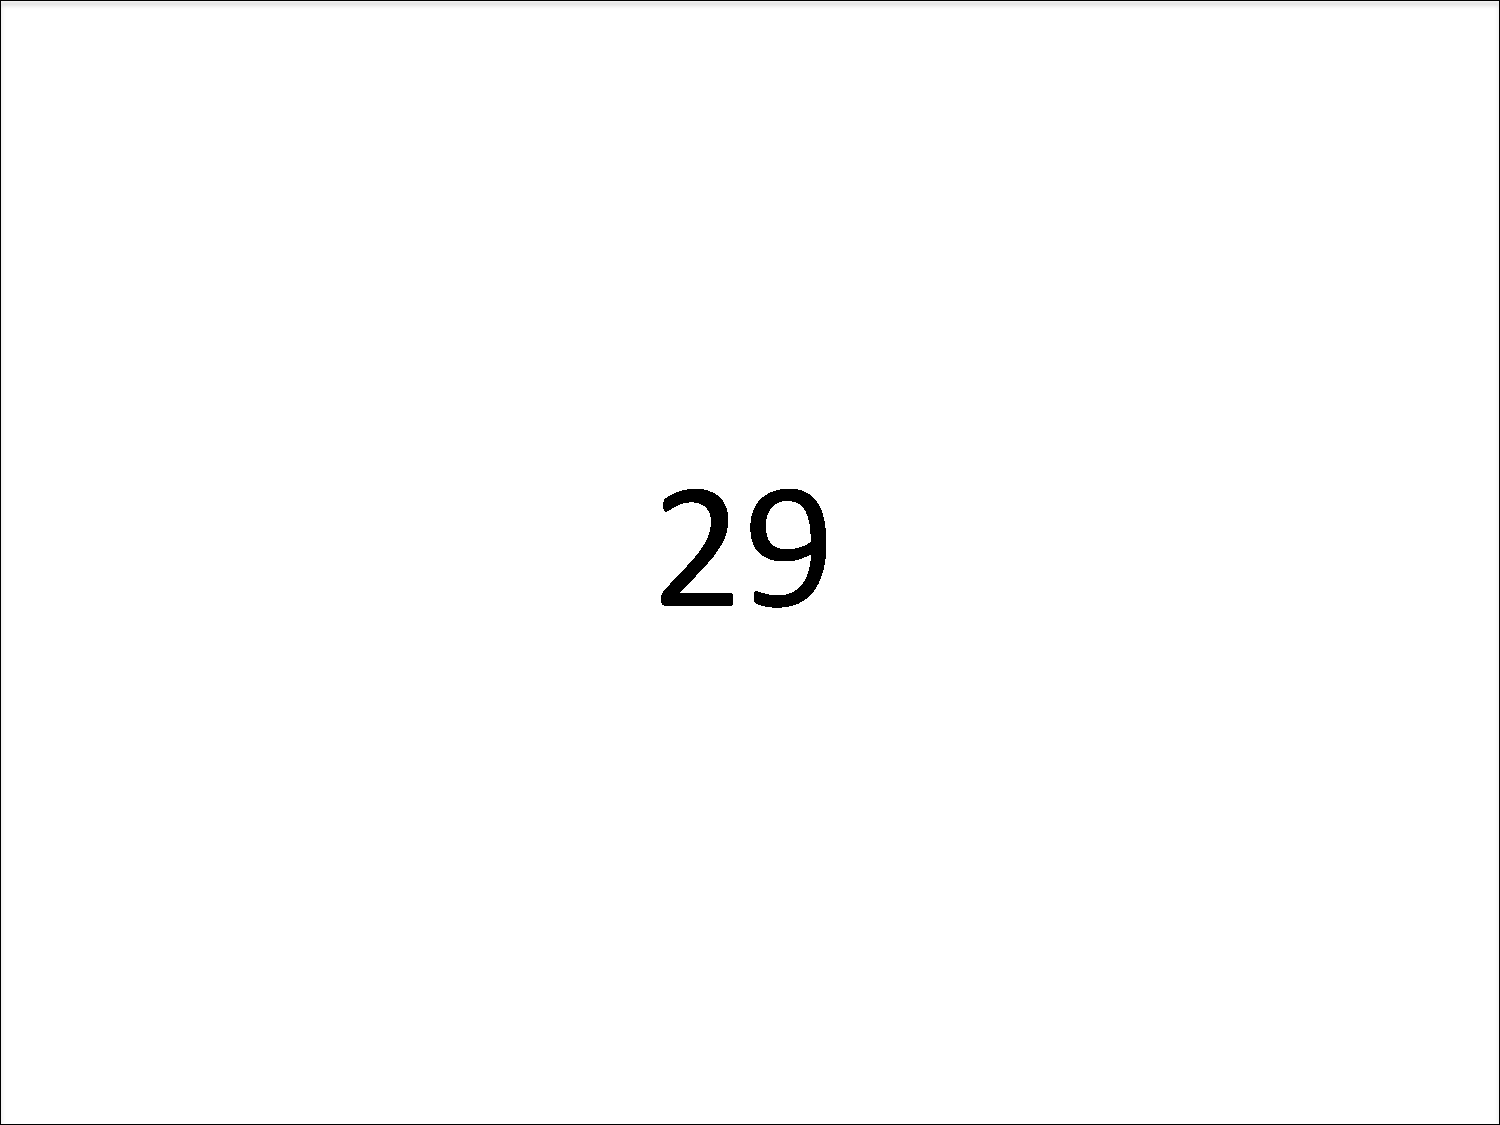
\includegraphics[width=0.19\textwidth]{images/partitioning1h.pdf}\vspace{1mm}
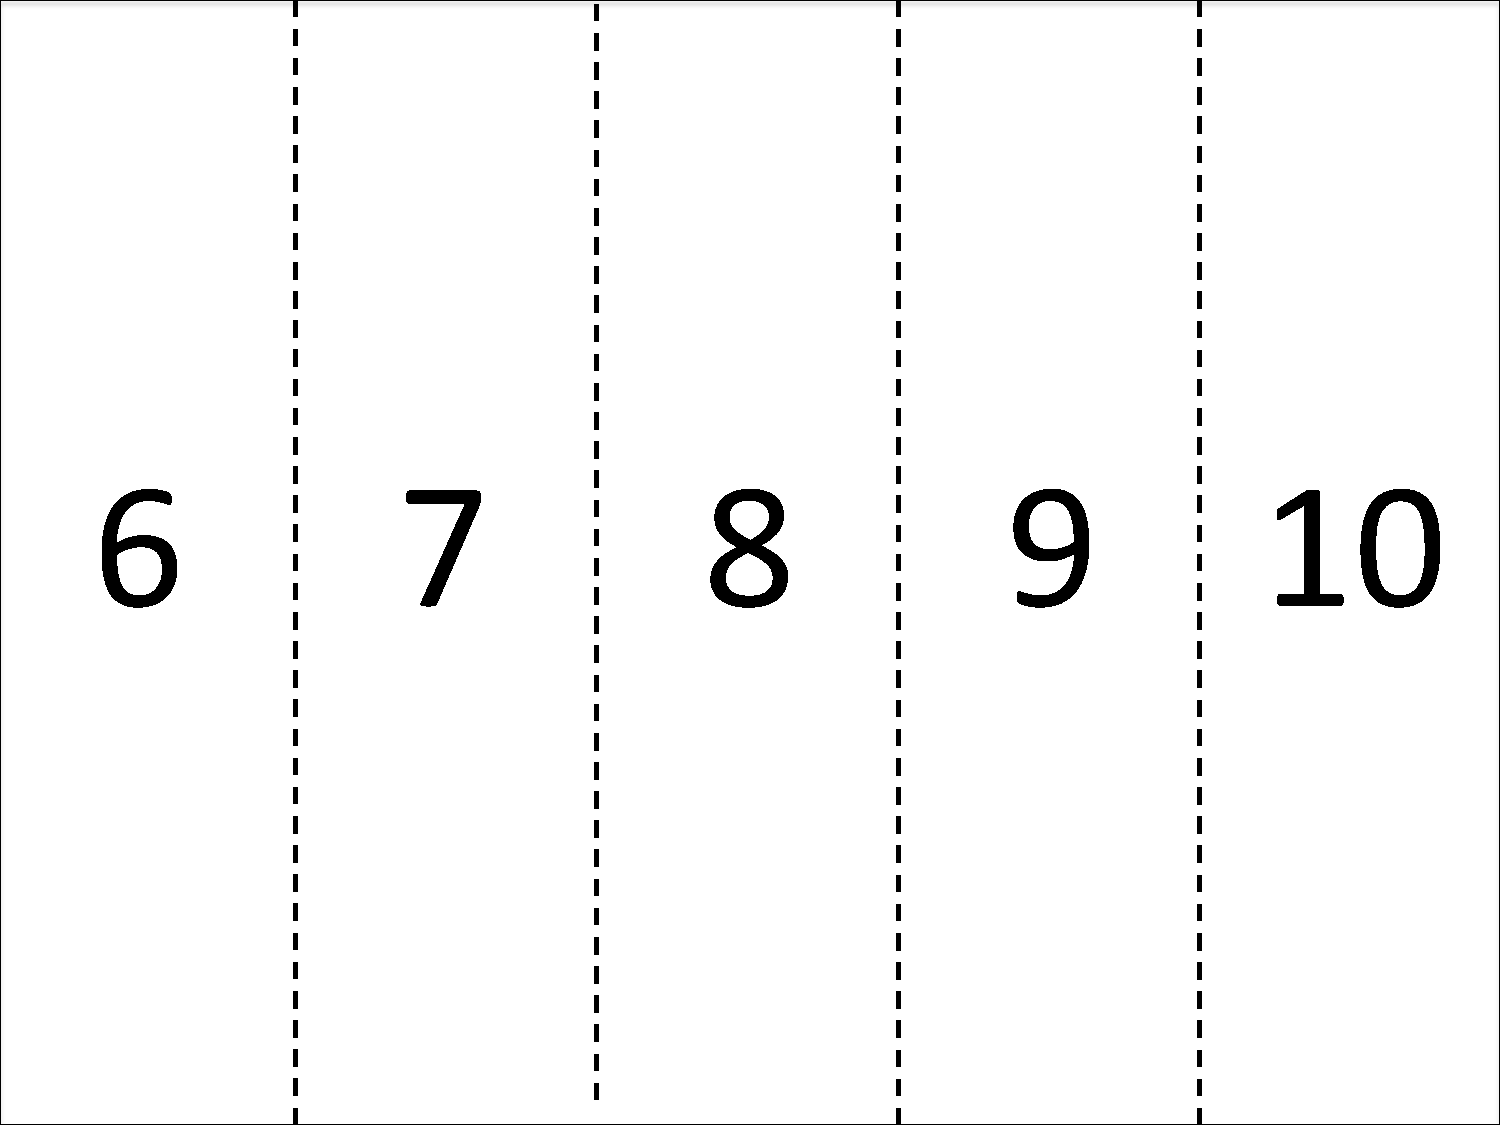
\includegraphics[width=0.19\textwidth]{images/partitioning5v.pdf}
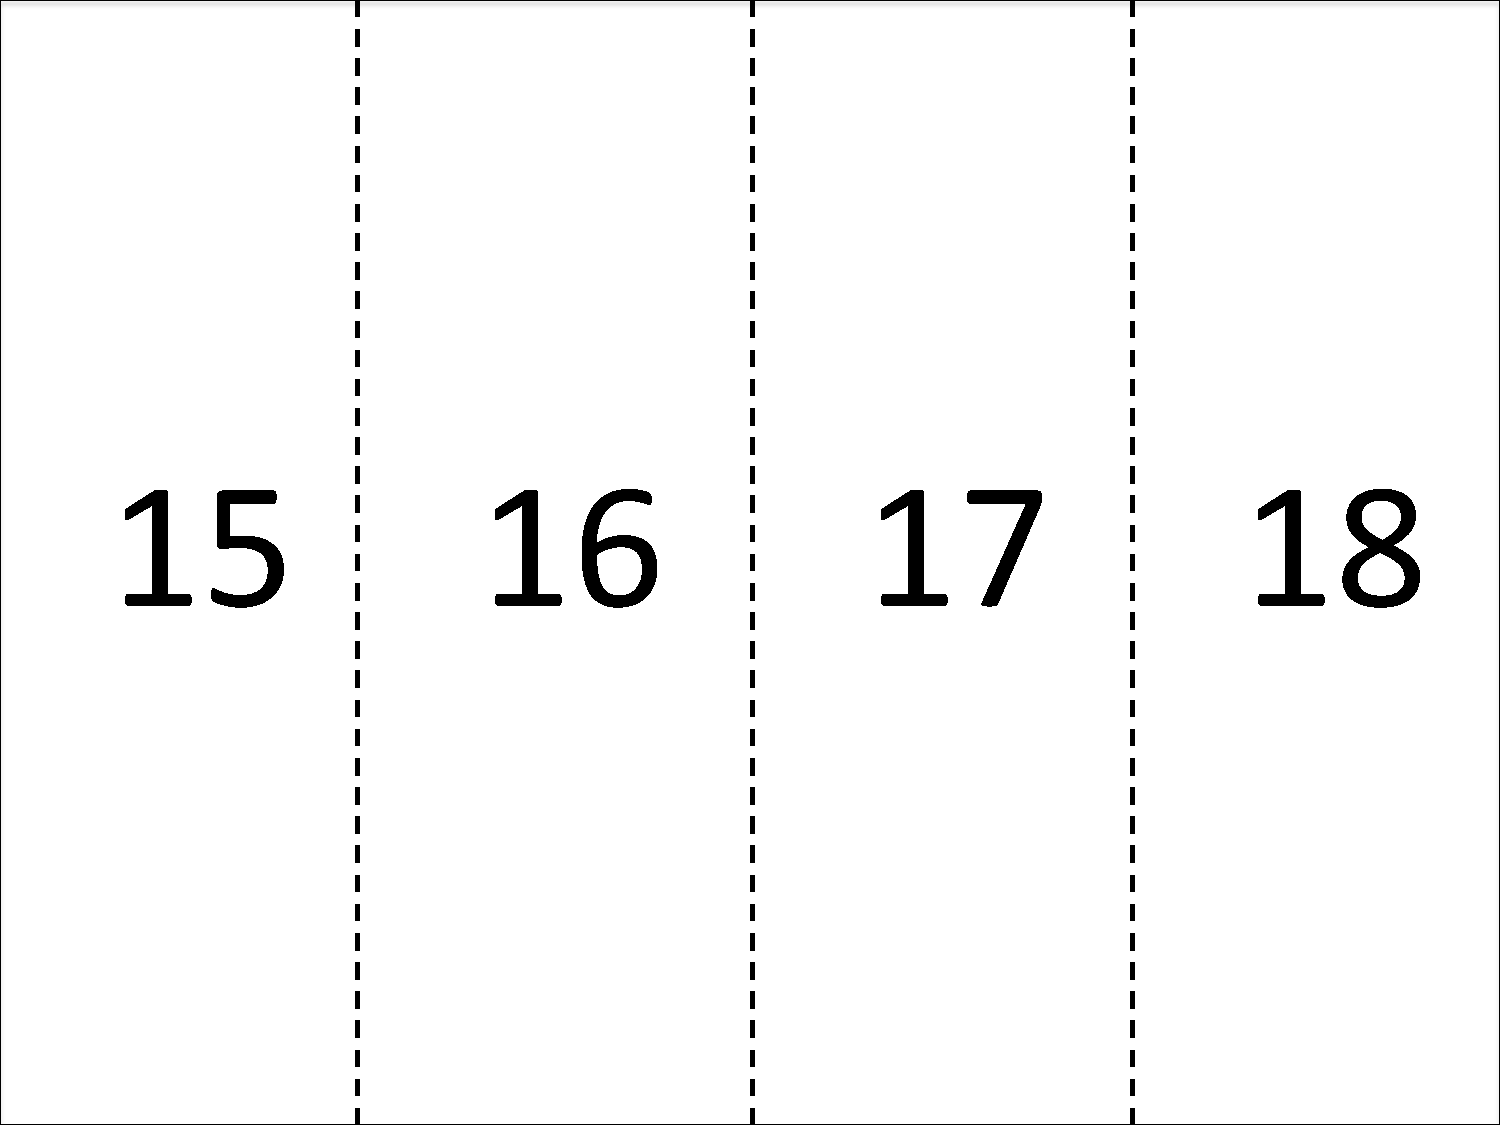
\includegraphics[width=0.19\textwidth]{images/partitioning4v.pdf}
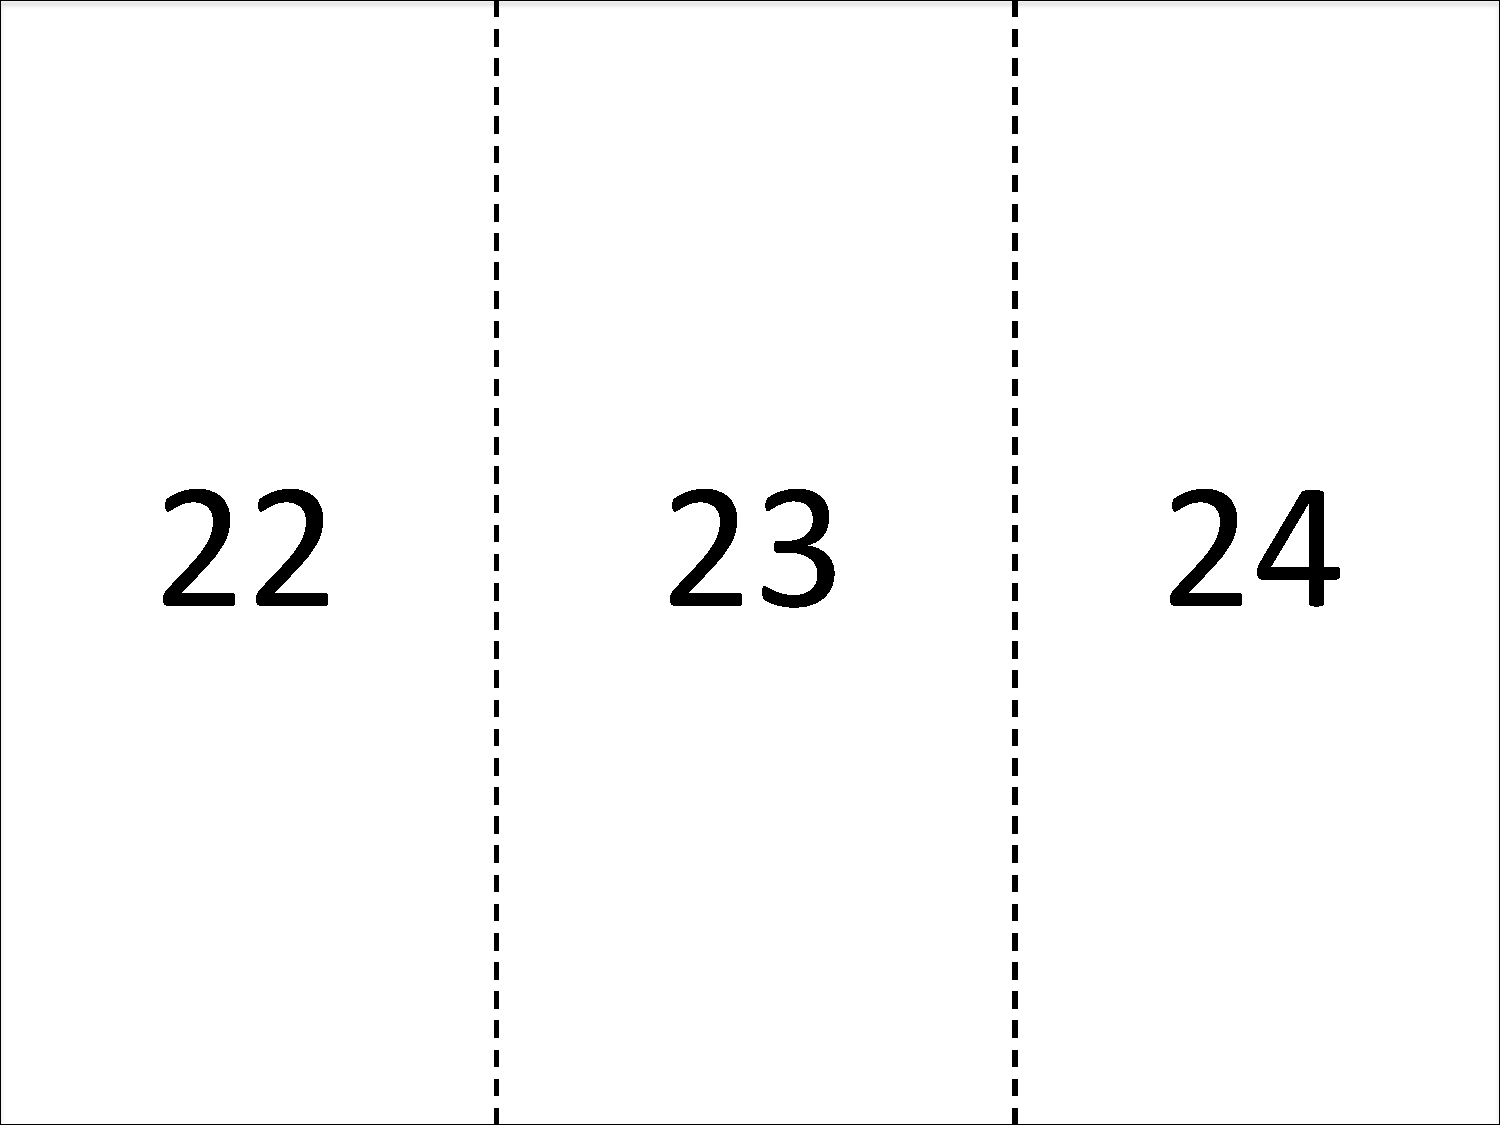
\includegraphics[width=0.19\textwidth]{images/partitioning3v.pdf}
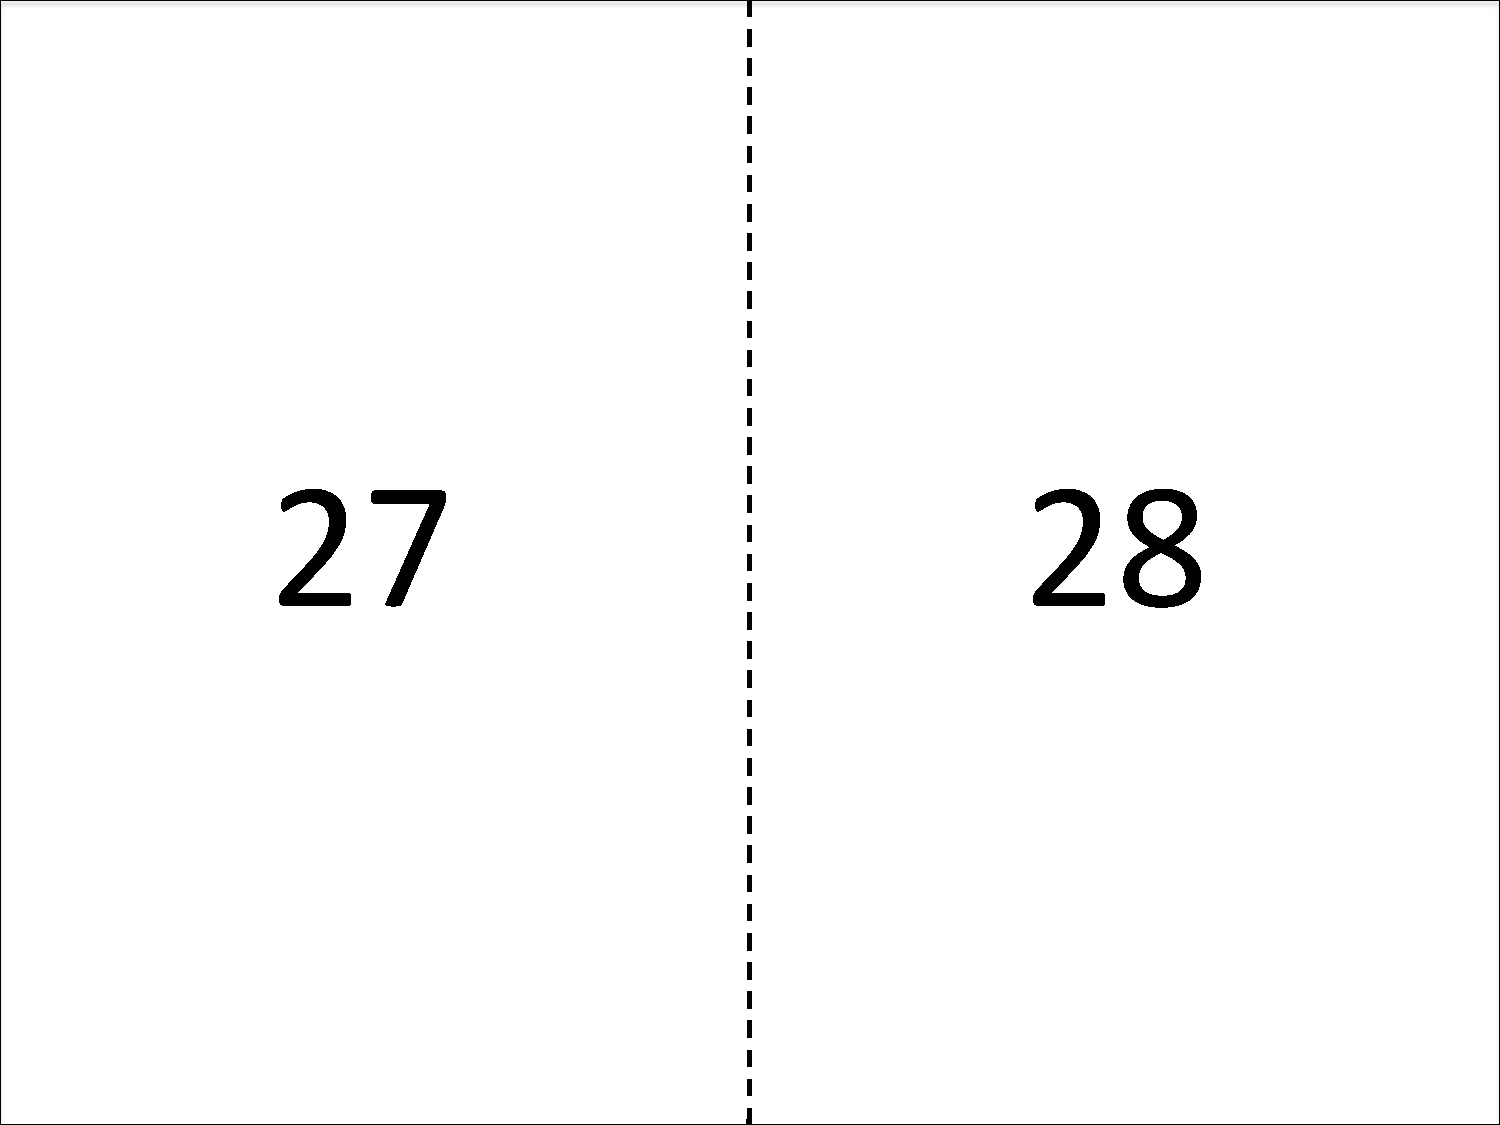
\includegraphics[width=0.19\textwidth]{images/partitioning2v.pdf}
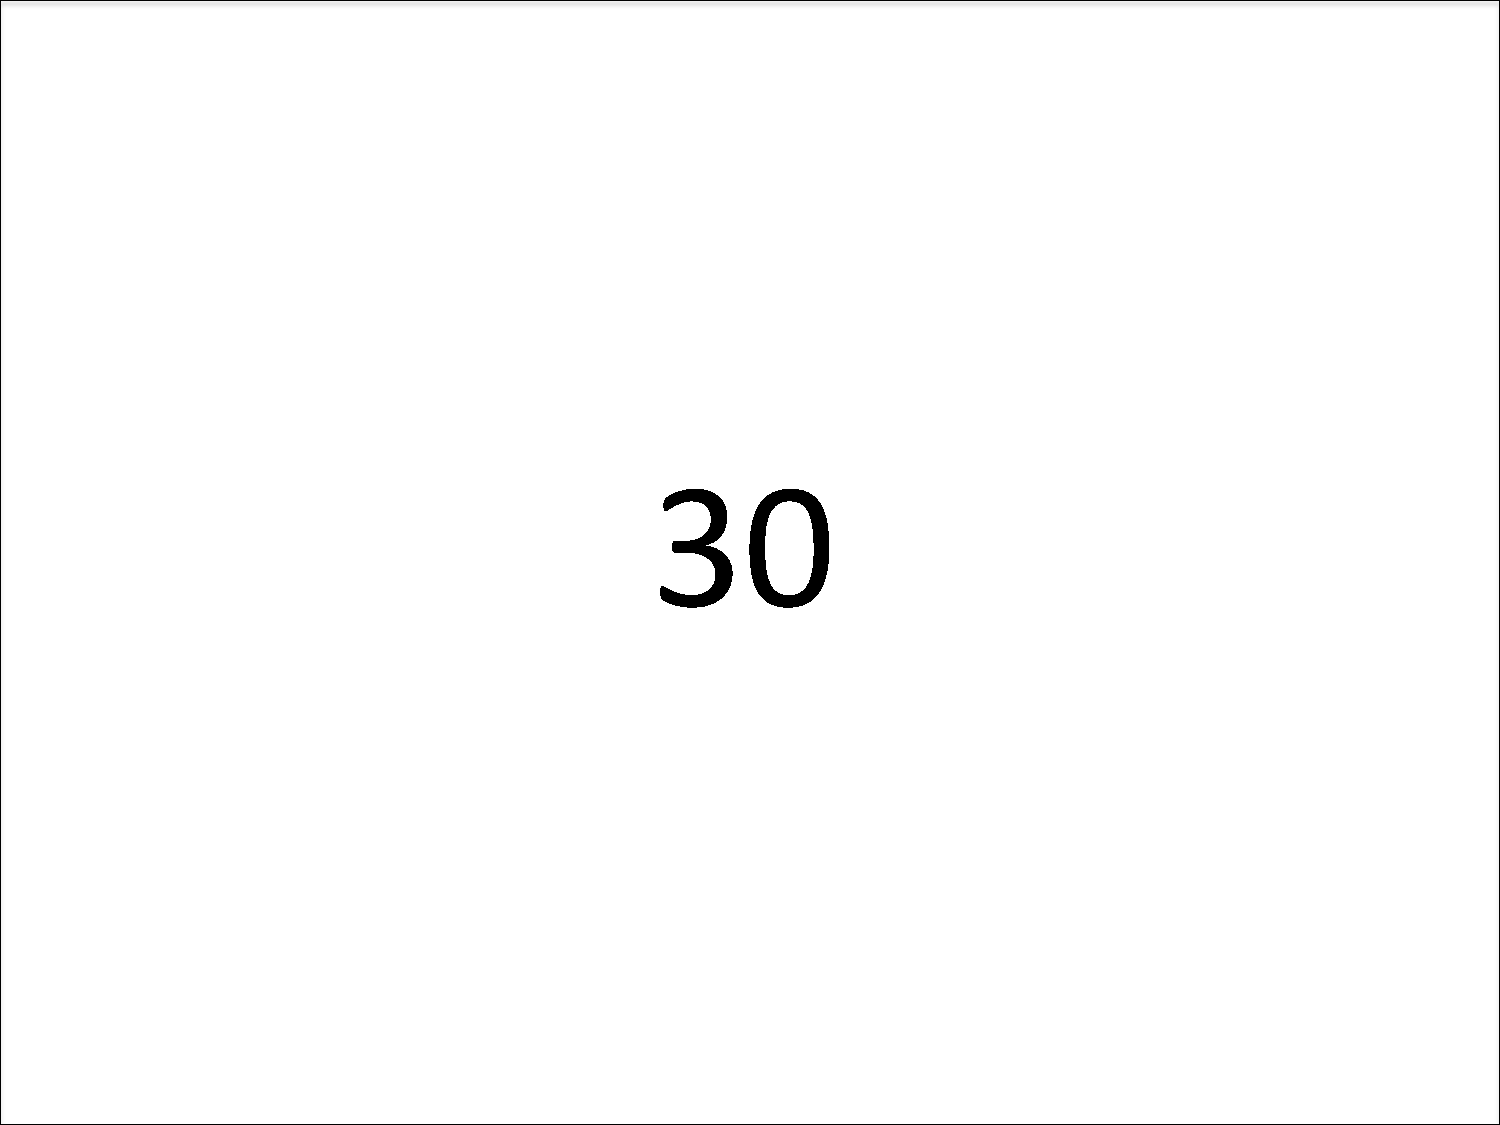
\includegraphics[width=0.19\textwidth]{images/partitioning1v.pdf}
\caption{Pyramidal image splitting for feature extraction}
\label{fig_partitioning}
\end{figure}


\subsubsection{Clustering}
A first, rather naive approach to clustering the visual characteristics extracted would be to concatenate the feature vectors (histograms), and apply one of the established clustering algorithms such as k-means.\index{K-Means} The fact that remains unseen in this approach is that, generally, the values of different features are usually measured on different scales and therefore vary in their orders of magnitude. They also consist of a different number of dimensions. \\
These circumstances influence any algorithm based on the distance between two images. Since differences in the larger values will usually be larger in its absolute value, they will also be more influential to the overall distance than the dimensions with smaller values. Furthermore, the feature with more dimensions will always be more influential.

\bigskip
So, instead, k-means is applied separately for colors and edges, and the results are later joined through \emph{late fusion}\index{Late Fusion}, as explained below. As no specific criteria exist for the number of clusters that should be achieved, k is chosen by the established rule of thumb: $ k = \sqrt{n/2} $ \cite[p.365]{mardia1979}, where $n$ is the number of items to be clustered. K-means was chosen over hierarchical clustering which is a recursive k-means approach \cite[p.17-20]{de2005hierarchical}, because it provided more well- and equally-sized clusters, the latter in hierarchical clustering often just splits off single images.\\
Initially, we planned to use an adaptive k, that is, start with a small k and increase it until the error (mean distance from centroids) no longer decreases. Despite its higher computation complexity, it does not seem to provide better results than the rule of thumb. For example in color clustering, the adaptive approach often just separates black and white images from colored ones.\\
We combine the single-feature clusters by intersecting them, which is a simple and performant late fusion method\index{Late Fusion}. It ensures that all images within a cluster are similar in color as well as edge structure and leads to less or equal to $ n/2 $ subclusters.

\newpage
%
\section{Evaluation}
\label{sec_evaluation}

We evaluated our tool on a set of 9,201 images, which are a subset of the 1 million images of the MIRFLICKR-1M\footnote{http://press.liacs.nl/mirflickr/} file set, and the query term ``food''. Since no comparable algorithms exist, the evaluation is mainly aimed at obtaining the best values for the parameters and at providing a basis for comparison of further improvements and future work.

\subsection{Test set}
\label{sec_testset}
No gold standard is available to tell us which pictures show food and how similar the images are. The creation of such standards and training data is exactly the task we want to facilitate with this work.\\ 
To test the quality of our algorithm, we wrote a tool allowing us a crowdsourced generation of the needed reference data by the general public. This was achieved in two phases:\\

First, the users were shown random picture out of the 9,201 test set images and asked whether it shows food or not. We normalized these answers, so that there is only one vote per user per picture. In the case a user rated a picture multiple times, the value is determined by the ratio of positive (\emph{``shows food''}) and negative (\emph{``does not show food''}) votes of each user on one picture. We consider all those images as showing food that received at least 50\% positive votes. With over 35,000 clicks by more than 20 participants, 1,142 images out of the total 9,201 images were identified to show food. \\

Since data on the semantic and visual similarity of these pictures is also necessary for the evaluation, in the second phase, the users were shown pairs of images, on which we knew from phase 1 that they contain food, and asked to compare them. They could choose between three levels of semantic similarity: \emph{not similar}, \emph{same object}, and \emph{same object and same context}, and two levels of visual similarity: \emph{similar}, and \emph{not similar}.\\
Among the 12,962 votes of more than 30 participants were 757 pairs of images with same objects, 345 pairs with same object and same context, as well as 1,854 pairs of visually similar images. Multiple votes on one pair were rare (39 cases), and therefore simply not taken into account if they contradicted each other.

\subsection{Quality Indicators}
The evaluation focuses on the following four main aspects of our algorithm:
\begin{enumerate}
\item Retrieval of matching images
\item Semantic hierarchy and clusters
\item Visual clustering
\end{enumerate}

We measure the quality of the image retrieval (\emph{1.}) by calculating the F-Measure for the returned pictures, comparing our algorithm's result to the crowdsourced generated test set of phase 1. \todo{should we compare synset detection mechanisms?} 

The quality of the hierarchy of the retrieved images (\emph{2.}) is based on the \emph{same object} and \emph{same object and context} pairs: The  minimal path distance for an annotated pair of pictures can be calculated and used to determine the closeness of two images: \[closeness(x,y) = 1/distance(x,y)\] Averaging this value over all pairs of a similarity category returns a value between 0 and 1 (below referenced as $c_o$ for same object pairs, $c_c$ for same object and same context pairs, and $c_n$ for not similar pairs), with the optimal values being 1 for positive (similar) pairs, and 0 for negative (non-similar) pairs. 
We include the keyword clustering in this evaluation by handling the clusters in a node as its children. Consequentially, the perfect score of 1 can only be reached when two semantically similar images are not only in the same node but also in the same semantic subcluster.

Visual similarity (\emph{3.}) is evaluated on the whole test set, because not enough comparison data is available to get valuable results if only comparisons within semantic clusters were used. Once again, F-Measure is used as indicator.

\todo{vary parameters given by frontend, trying to find best configuration}

\subsection{Results}
\label{sec_results}

\subsubsection*{Image Retrieval}

Our image retrieval has a precision of 50.2\% and recall of 85.9\% on the ``food'' query, before execution of the semantic clustering that removes outliers. Without the use of co-occurring tags described in section \ref{sec_picturestonodes}, both values show no significant difference with p = 50.5\% and r = 85.4\%.
After the semantic clustering, the measures depend on the  parameters \emph{minimal node size}, \emph{mcl clustering threshold}, and \emph{minimal mcl cluster size}, described in sections \ref{sec_picturestonodes} and \ref{sec_keywordclustering}. The results for different values of this parameter are presented in table \ref{tab_retrievalevaluation}.\\

\begin{table}[h]
   \begin{tabular}{| p{2.2cm}| p{2.2cm}| p{2cm} || p{2cm} | p{2cm} | p{2cm} |}
    \hline
    \emph{mcl clustering threshold} & \emph{minimal mcl cluster size} & \emph{minimal node size} & \emph{precision} & \emph{recall} & \emph{f-measure} \\ \hline
    0 	& 0 	& 0 & 0.501532 & 0.859143 & 0.633344 \\ \hline
    0 	& 5 	& 0 & 0.559668 & 0.783036 & 0.652773 \\ \hline
    5 	& 5 	& 5 & 0.549815 & 0.798214 & 0.651129 \\ \hline     
    15 	& 25 &  5 & 0.615894 & 0.747321 & 0.675272 \\ \hline
    15 	& 10 & 15 & 0.585333 & 0.783929 & 0.670229 \\ \hline
    15 	& 25 & 15 & 0.695298 & 0.672791 & 0.683859 \\ \hline
    	100 	& 100 & 100 & 0.757858 & 0.569554 & 0.650350 \\ \hline
    \end{tabular}
    \caption{Precision and recall of the image retrieval}
	\label{tab_retrievalevaluation}
\end{table}


\subsubsection*{Semantic Hierarchy and Clusters}

The results of the semantic hierarchy and cluster evaluation also depend on the parameters mentioned for image retrieval. The measurements listed in table \ref{tab_treeevaluation} indicate that the best distinction between images showing the same objects and images showing different objects is achieved with low \emph{minimal mcl cluster size}, that is, without outlier removal. The other parameters' values correlate with those of the image retrieval evaluation above.\\

\begin{table}[h]
    \begin{tabular}{| p{2.2cm} | p{2.2cm} | p{2cm} || p{1.4cm} | p{1.4cm} | p{1.4cm} | p{1.4cm} |}
	\hline    
    \emph{mcl clustering threshold} & \emph{minimal mcl cluster size} 	& \emph{minimal node size} & $c_o $ & $c_c$ & $c_n$ & $c_o - c_n$ \\ \hline
    0 	& 0 	& 0 & 0.25075 & 0.25483 & 0.23430 & 0.01645 \\ \hline
    0 	& 5 	& 0 & 0.25707 & 0.26691 & 0.24857 & 0.00850 \\ \hline
    5 	& 5 	& 5 & 0.26129 & 0.27160 & 0.25347 & 0.00782 \\ \hline     
    15 	& 25 &  5 & 0.24118 & 0.24927 & 0.23345 & 0.00773\\ \hline
    15 	& 0 & 15 & 0.27757 & 0.28242 & 0.25897 & 0.01860 \\ \hline
    15 	& 10 & 15 & 0.28285 & 0.29194 & 0.26884 & 0.01401 \\ \hline
    15 	& 25 & 15 & 0.28571 & 0.29391 & 0.27563 & 0.01008 \\ \hline
    	100 	& 100 & 100 & 0.32578 & 0.34126 & 0.31711 & 0.00867 \\ \hline
    \end{tabular}
    \caption{Semantic quality measures}
	\label{tab_treeevaluation}
\end{table}

It can generally be observed that varying the parameters most strongly influences the amount of the closeness measures, that is, all their values rise or drop somewhat consistently.
 
\subsubsection*{Visual Clustering}



\newpage
%
\section{Zusammenfassung\index{Zusammenfassung} und Ausblick}
\label{sec_conclusion}

Das Kapitel "`Zusammenfassung und Ausblick"' soll die gewonnenen Ergebnisse und Erkenntnisse Ihrer Arbeit knapp zusammenzufassen.
Stellen Sie dabei eindeutig klar, was wichtig ist und was nicht.
Dazu z�hlt auch, dass Sie einen Ausblick\index{Ausblick} auf die Weiterentwicklung innerhalb des von Ihnen bearbeiteten Themengebiets geben k�nnen.
\begin{itemize}
\item Was haben wir erreicht?
\item Was sind die n�chsten Schritte?
\item Wie k�nnen die gewonnenen Ergebnisse angewendet werden?
\item Warum sind die gewonnenen Ergebnisse bedeutend?
\end{itemize}

\newpage
%
\section{Future Work}
\label{sec_future}

How to improve, what other approaches to take


%% Anh�nge
\newpage
\begin{appendix}


\section{Glossary} %Appendix (Glossar)

\begin{description}
\item[Synset:]\index{Synset} 

\item[Wordnet:]\index{Wordnet} 

\item[Beispiel:]\index{Beispiel} eine Beispiel-Erkl�rung

\end{description}


\newpage

% Appendix (Akronyme)
\section{Abbreviations and Acronyms}\index{Akronyme}

\begin{tabbing}
\hspace*{3cm}\=  \\ \kill

Bsp \> Beispiel\\

\end{tabbing}


\end{appendix}


%Hier kommt das Literaturverzeichnis
\newpage

\addcontentsline{toc}{section}{References} % Zeile f�r das Inhaltsverzeichnis

\bibliographystyle{alpha}
\bibliography{bibfile}

\newpage

%Hierhin kommt der Index (Sachverzeichnis)
\addcontentsline{toc}{section}{Index} % Dies ist die Zeile f�r das Inhaltsverzeichnis
\flushbottom
\printindex

\end{document}
